\documentclass[titlepage]{jsarticle}
\usepackage[dvipdfmx]{graphicx}
\usepackage{h31ec-exp}
\makeatletter
\newcommand{\figcaption}[1]{\def\@captype{figure}\caption{#1}}
\newcommand{\tblcaption}[1]{\def\@captype{table}\caption{#1}}
\makeatother
\title{光センサの使い方}
\grade{3年32番}
\author{平田 蓮}
\team{第10班}
\date{2019年7月22日}
\expdate{2019年7月1日, 7月8日, 7月22日}
\coauthor{
    8番 & 小林 歩夢 \\
    21番 & 相馬 拓杜 
}
\begin{document}
\maketitle
\section{目的}
    どのような制御システムでも, ~制御対象の現在の状態を知って次の適切な
    操作を決めるために, ~状態を計測するセンサが不可欠である. ~ここでは
    光センサの使い方について学ぶ.

    2種類の光センサを使用して, ~その特徴や基礎特性をまず理解する.
    ~次にセンサとして使用するための回路について検討し, ~その応用技術
    を身に付ける.

\section{光センサの種類と選定}
    光センサといっても様々な種類がある. ~例えば, ~フォトダイオード,
    ~フォトトランジスタ, ~光導電素子(CdSセル), ~焦電素子, ~光電管,
    ~カラーセンサ, ~個体イメージセンサ(CCD)などがある. ~光センサの検出対象
    として, 「近赤外線, ~可視光線, ~紫外線といったどの波長を検出するのか?」
    また, 「どのような応答速度が必要なのか?」等の要因が重要になる.
    ~言い換えれば, ~検出対象の特性によって光センサの選定をする必要がある.

\section{CdS光導電セル}
    \subsection{構造と原理}
        CdSセルは流下カドミウムを主成分とした光導電素子の一種であり,
        ~照射光によって内部抵抗が変化する一種の光抵抗器と考えることができる.
        照射光が強くなるとその内部抵抗は低下する.

        図\ref{fig:CdS}にCdSセルの回路記号を示す. ~CdSセルは
        その性質上応答速度が非常に遅く, ~高速の光スイッチングには不向きである.
        ~その為, ~用途は緩やかな照度変化のセンシングに限定される.
        
        また, ~CdSセルには極性がない.

        \begin{figure}[ht]
            \centering
            %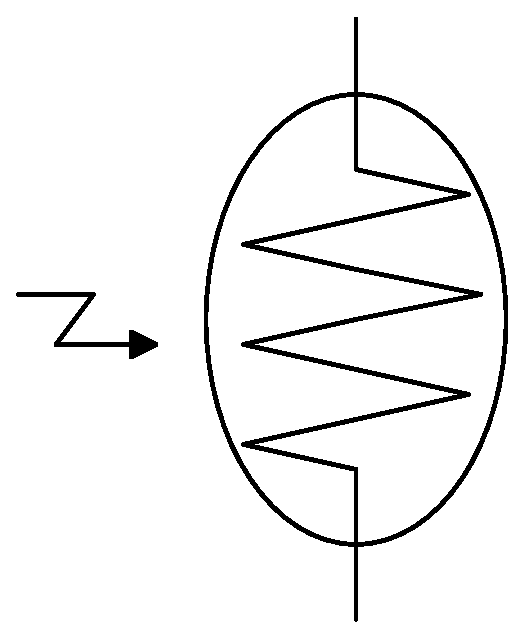
\includegraphics{images/CdS.eps}
            \caption{CdSセル回路記号}
            \label{fig:CdS}
        \end{figure}

    \subsection{基礎特性}
        光源にLEDを用いて, ~照射光の強さによりCdSセルの抵抗値が変化
        することを確認する. ~なお, ~LEDに流れる電流と発光強度は正比例
        しない.

        \subsubsection{実験方法}
            \begin{enumerate}
                \item 図\ref{fig:基礎特性}のように配線を行う.
                \item 電源電圧を0[V]から徐々にあげると電流$I_F$が
                    増加し, ~LEDの明るさが変化することと, ~同時に
                    CdSの抵抗値$R_C$が変化していることを確認する.
                \item 組立済回路部分に暗幕を被せ光を遮断し,
                    ~電源電圧を変化させ, ~$I_F$が1[mA]から20[mA]
                    の時の$R_C$を測定し, ~表にまとめる.
                \item 作成した表より, ~$I_F$-$R_C$グラフを両対数グラフ
                    で作成する.
            \end{enumerate}

            \begin{figure}[ht]
                \centering
                %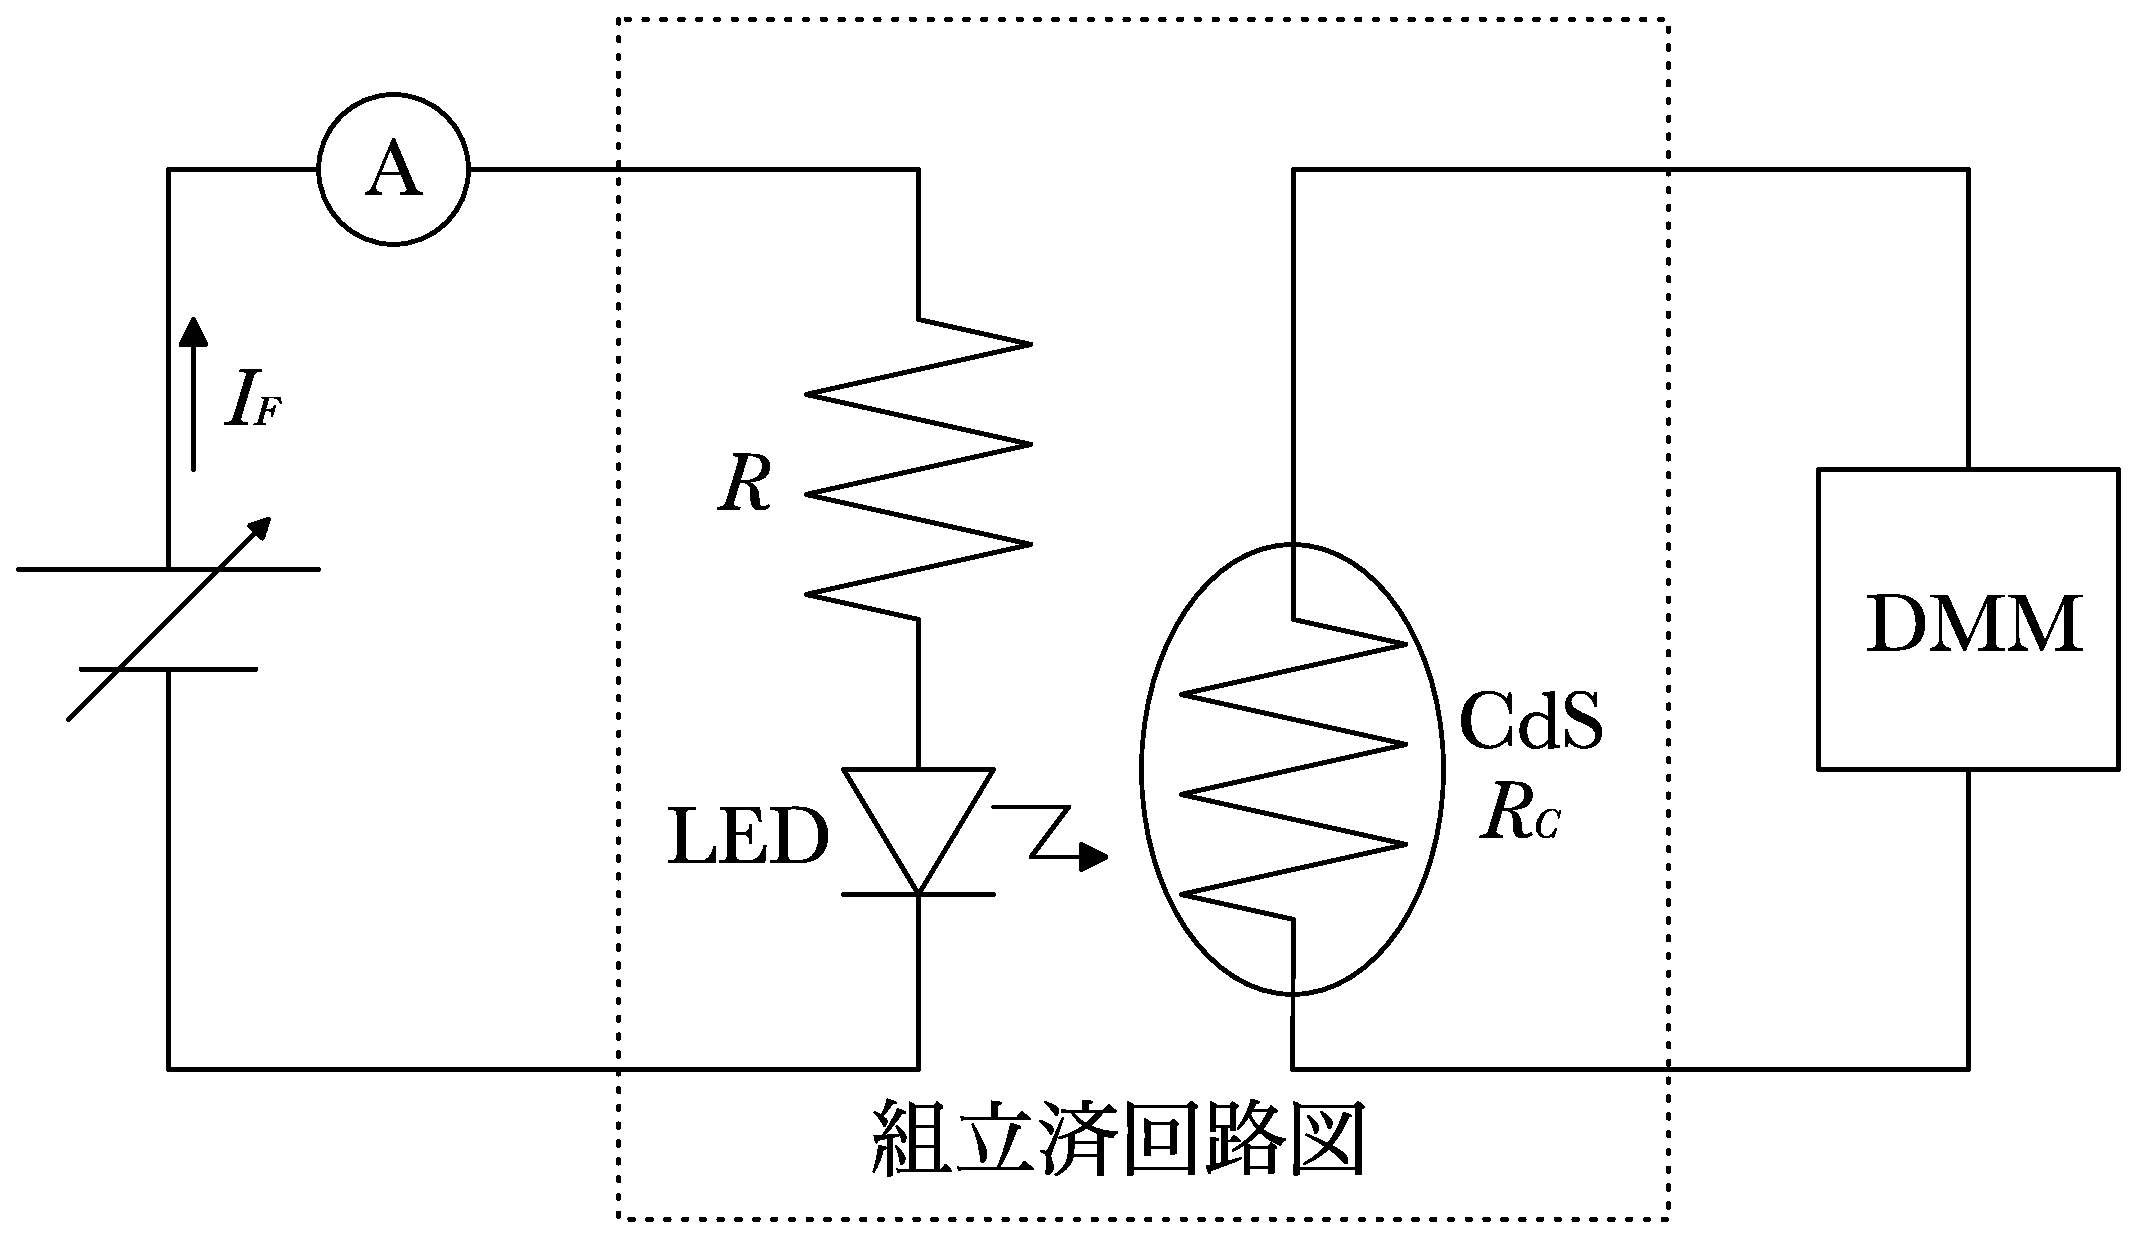
\includegraphics{images/CdS_circuit.eps}
                \caption{CdSセル基礎特性測定回路}
                \label{fig:基礎特性}
            \end{figure}

            \paragraph{使用素子 $\cdot$ 使用器具}
                \begin{description}
                    \setlength{\leftskip}{1.5em}
                    \item[組立済回路] CDS-A1
                    \item[CdSセル] MKY-54C348
                    \item[LED] L-513SGT3
                    \item[デジタルマルチメータ] EC-12
                    \item[直流電源] Ec-01
                    \item[電流計] 341 
                \end{description}
                

        \subsubsection{結果}
            図\ref{tab:基礎特性結果}, \ref{fig:基礎特性グラフ}
            に結果の表とグラフを示す.

            \begin{figure}[ht]
                \def\@captype{table}
                \begin{minipage}{0.5\hsize}
                    \begin{center}
                        \caption{基礎特性測定結果}
                        \label{tab:基礎特性結果}
                        \begin{tabular}{c|c}
                            
                        \end{tabular}
                    \end{center}
                \end{minipage}
                \begin{minipage}{0.5\hsize}
                    \begin{center}
                        %\includegraphics[width=8cm]{graphs/kisotokusei.pdf}
                        \caption{基礎特性グラフ(両対数)}
                        \label{fig:基礎特性グラフ}
                    \end{center}
                \end{minipage}
            \end{figure}

    \subsection{明暗判定回路} \label{明暗判定回路}
        CdSセルを用いて, ~暗くなったら赤色LEDを点灯させる簡単な回路を
        作成してみる.

        \subsubsection{実験方法}
            \begin{enumerate}
                \item 図\ref{fig:判定回路}のように配線を行う.
                    ~$VR$は10[k$\Omega$]の半固定抵抗とし,
                    ~$R$は1[k$\Omega$]の炭素皮膜抵抗とする.
                    ~また, ICには5[V]の電源電圧を供給する.
                \item CdSセルに蛍光灯の光が当たっている場合には
                    LEDが消灯し, ~CdSに当たっている光が遮断された
                    場合にはLEDが点灯するように$VR$を調節する.
            \end{enumerate}

            \begin{figure}[ht]
                \centering
                %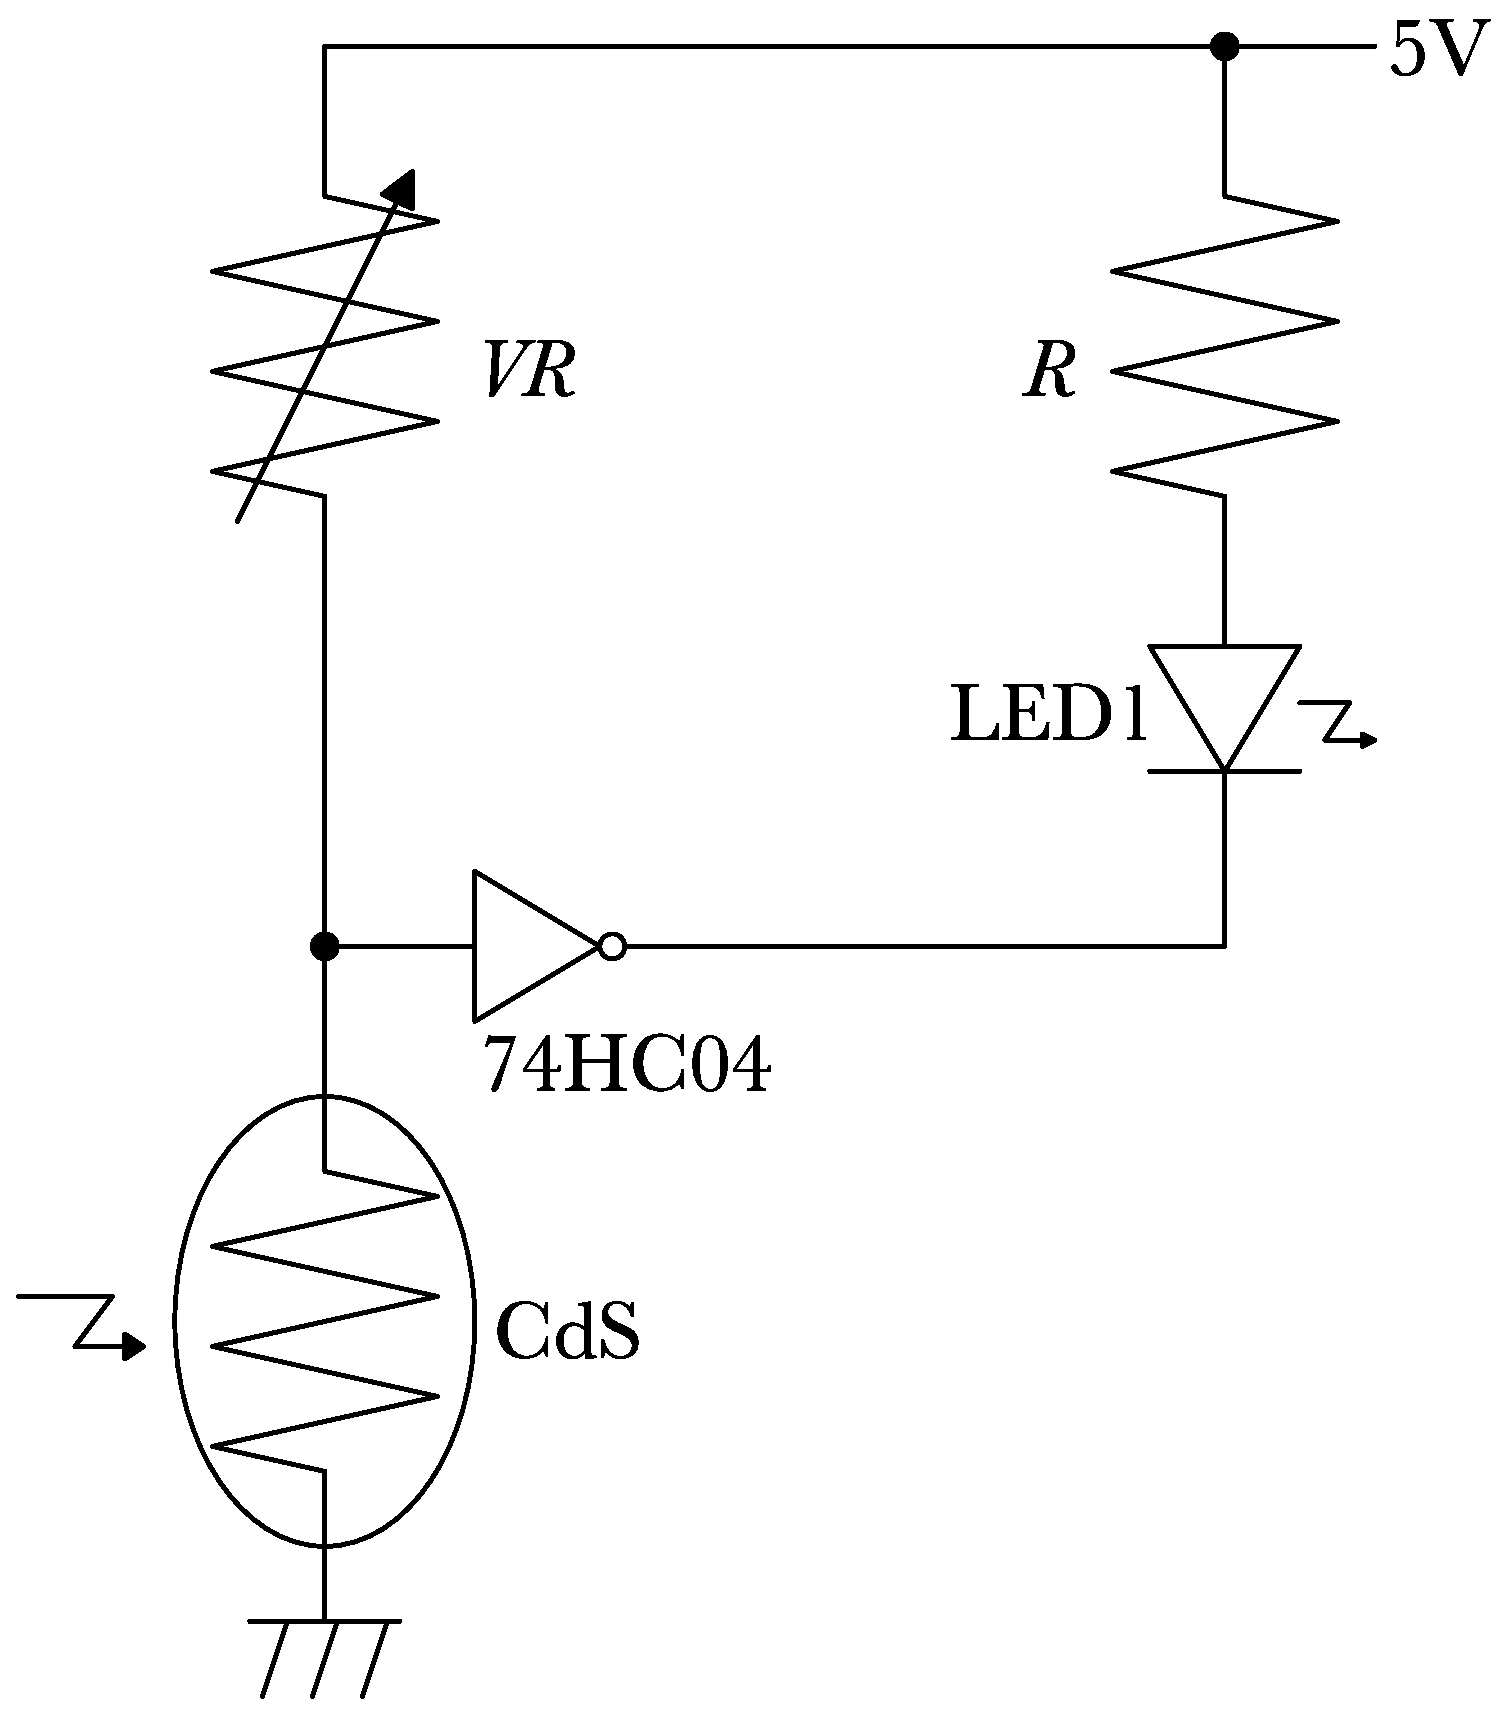
\includegraphics{images/hanteikairo.eps}
                \caption{明暗判定回路}
                \label{fig:判定回路}
            \end{figure}

            \paragraph{使用素子 $\cdot$ 使用器具}
                \begin{description}
                    \setlength{\leftskip}{1.5em}
                    \item[CdSセル] MKY-54C348
                    \item[LED] L-513LE1T
                    \item[IC] 74HC04
                    \item[デジタルマルチメータ] EC-12
                    \item[直流電源] Ec-01
                    \item[ブレッドボード] EC-16 
                \end{description}

        \subsubsection{結果 $\cdot$ 考察} \label{明暗判定考察}
            CdSセルに指をかざすとLEDが点灯し, ~指を離すと再び点灯した.

            これは, ~光が遮断されることでCdSの抵抗値が増え, ~C点での
            電圧が高くなり, ~NOTを通したB点の電圧が低くなり, ~A-B間に
            電位差が生まれるためである.

    \subsection{応用回路}
        CdSセルに蛍光灯の光が当たっている場合には緑色のLEDを点灯させ,
        ~CdS暗幕で覆った場合には赤色のLEDを点灯させる回路を設計$\cdot$
        作成してみる. ~\ref{明暗判定回路}節を参考にすると簡単に設計することが
        できる.

        ただし, ~使用器具は\ref{明暗判定回路}節と同様で,
        ~素子は以下のものを使用する.

            \paragraph{使用素子}
                \begin{description}
                    \setlength{\leftskip}{1.5em}
                    \item[CdSセル] MKY-54C348
                    \item[LED1(赤色)] L-513LE1T
                    \item[LED2(緑色)] L-513SGT3
                    \item[IC] 74HC04
                    \item[半固定抵抗(1個)] 10[k$\Omega$]
                    \item[炭素皮膜抵抗(2個)] 1[k$\Omega$]
                \end{description}

        \subsubsection{設計 $\cdot$ 組立}
            図\ref{fig:応用回路}に設計した回路図を示す.
            
            \begin{figure}[ht]
                \centering
                %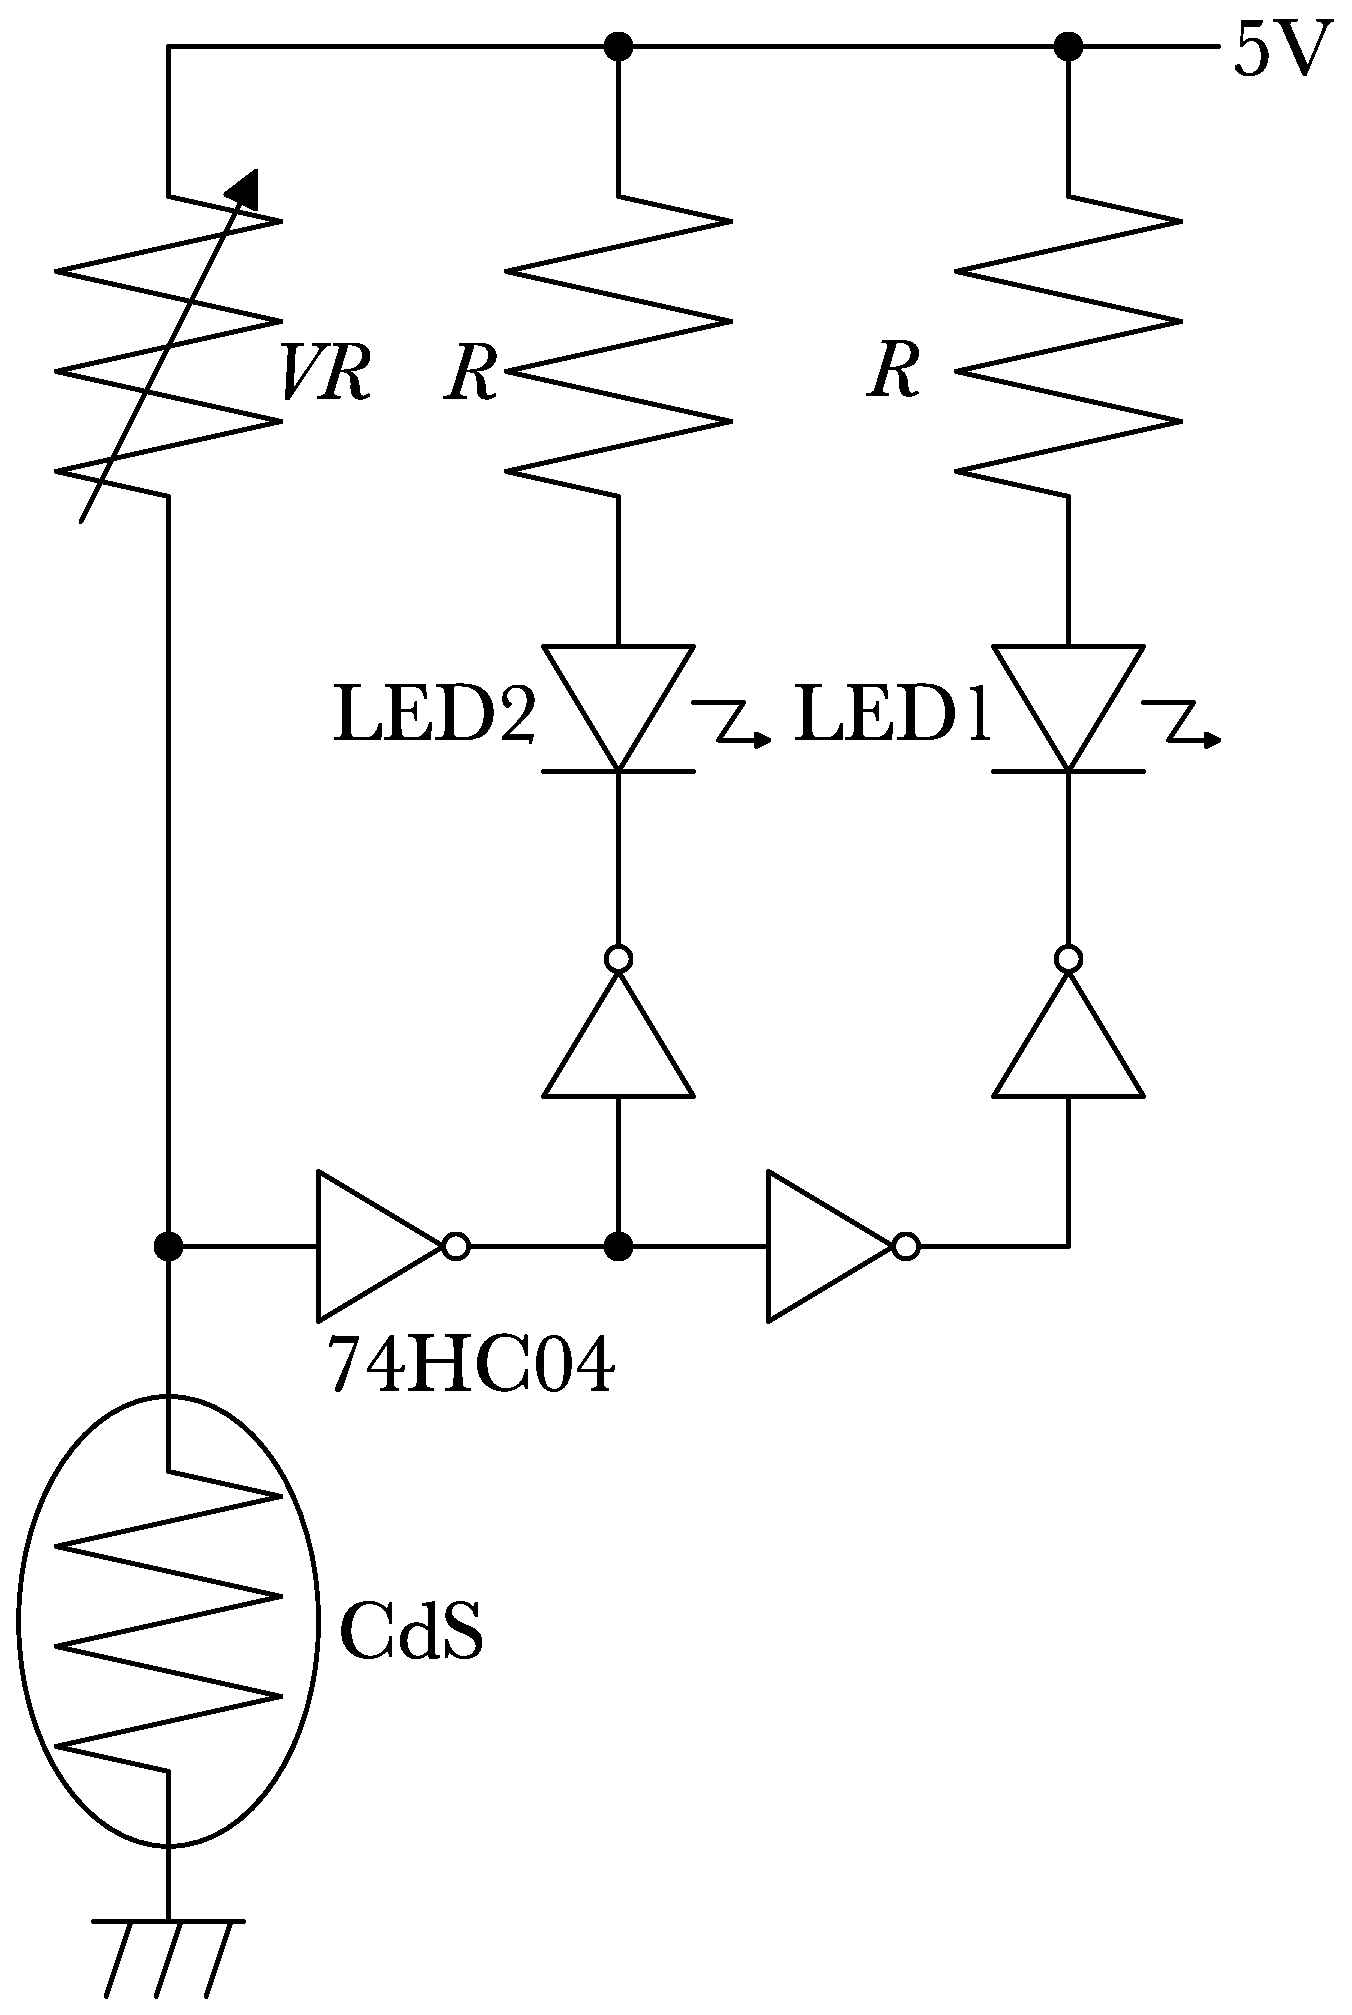
\includegraphics{images/ouyoukairo.eps}
                \caption{応用回路}
                \label{fig:応用回路}
            \end{figure}

            図\ref{fig:判定回路}の赤色LEDに並列に緑色LEDを接続し,
            NOT素子を挟むことで赤色と動作を反転させる.

            また, ~二つのLEDに流れる電流に差を生じさせないために,
            ~赤色LED側にもNOTを二つ挟んだ.
        
        \subsubsection{結果 $\cdot$ 考察}
            動作確認をしたところ, ~設計した回路は想定通りに動作した.
            
            この回路は, ~\ref{明暗判定考察}節に記したように
            赤色LEDが動作する. ~緑色LEDは赤色LEDと反転動作をするので,
            ~CdSに光が当たっている時のみ点灯する.

\section{フォトダイオード}
    \subsection{構造と原理} \label{フォトダイオード構造と原理}
        フォトダイオード(PD)は, ~半導体のPN接合に光が当たると電位差が
        生じる光起電力を利用したものである. ~PDはそれ自身起電力を有する
        素子であるため, ~動作させる場合に外部電源を必要としない.
        ~そのため, ~電源が無くても簡単な光検出回路を構成することができるが,
        ~その出力信号は極めて微弱であるため, ~一般的には
        何らかの増幅手段を併用する.
        
        なお, ~PDは入射光量と
        出力電流の線型性が優れており, ~CdSセルに比べ応答速度が100倍以上
        早い特徴がある.
        
        図\ref{fig:PD}にPDの回路記号を示す.

        \begin{figure}[ht]
            \centering
            %\includegraphics{images/PD.eps}
            \caption{PD回路記号}
            \label{fig:PD}
        \end{figure}

    \subsection{短絡特性} \label{短絡特性}
        光源にLEDを用いて, ~照射光の強度によりPDの光起電力が変化する
        ことを確認する. ~なお, ~LEDに流れる電流と発光強度は正比例しない.

        \subsubsection{実験方法}
            \begin{enumerate}
                \item 図\ref{fig:短絡特性回路}のように配線を行う.
                    ~電流計$A_1$, $A_2$にはデジダルマルチメータを
                    使用する.
                \item 電源電圧を0[V]から徐々にあげると電流$I_F$が
                    増加し, ~LEDの明るさが変化することと, ~同時に
                    $I_S$が変化していることを確認する.
                \item 組立済回路部分に暗幕を被せ光を遮断し,
                    ~電源電圧を変化させ, ~$I_F$が5[mA]から20[mA]
                    の時の$I_S$を測定し, ~ 表にまとめる.
                \item 作成した表より, ~$I_F$-$I_S$グラフを両対数グラフ
                    で作成する.
            \end{enumerate}

            \begin{figure}[ht]
                \centering
                %\includegraphics{images/PD_short_circuit.eps}
                \caption{PD短絡特性測定回路}
                \label{fig:短絡特性回路}
            \end{figure}
            
            \paragraph{使用素子 $\cdot$ 使用器具}
                \begin{description}
                    \setlength{\leftskip}{1.5em}
                    \item[組立済回路] PD-A3
                    \item[PD] S1133
                    \item[LED] L-513SGT3
                    \item[デジタルマルチメータ] EC-21, EC-23
                    \item[直流電源] Ec-11
                \end{description}

        \subsubsection{結果}
            図\ref{tab:短絡特性結果}, \ref{fig:短絡特性グラフ}
            に結果の表とグラフを示す.

            \begin{figure}[ht]
                \def\@captype{table}
                \begin{minipage}{0.5\hsize}
                    \begin{center}
                        \caption{短絡特性測定結果}
                        \label{tab:短絡特性結果}
                        \begin{tabular}{c|c}
                            
                        \end{tabular}
                    \end{center}
                \end{minipage}
                \begin{minipage}{0.5\hsize}
                    \begin{center}
                        %\includegraphics[width=8cm]{graphs/tanrakukusei.pdf}
                        \caption{短絡特性グラフ(両対数)}
                        \label{fig:短絡特性グラフ}
                    \end{center}
                \end{minipage}
            \end{figure}

    \subsection{開放特性}
        ここでは\ref{短絡特性}節と対照的に,
        光の強度によりPDの開放電圧が変化することを確認する.
            
        \subsubsection{実験方法}
            \begin{enumerate}
                \item 図\ref{fig:開放特性回路}のように配線を行う.
                    ~電流計$A$, ~電圧計$V$にはデジダルマルチメータを
                    使用する.
                \item 電源電圧を0[V]から徐々にあげると電流$I_F$が
                    増加し, ~LEDの明るさが変化することと, ~同時に
                    $V_O$が変化していることを確認する.
                \item 組立済回路部分に暗幕を被せ光を遮断し,
                    ~電源電圧を変化させ, ~$I_F$が5[mA]から20[mA]
                    の時の$V_O$を測定し, ~表にまとめる.
                \item 作成した表より, ~$I_F$-$V_O$グラフを片対数グラフ
                    で作成する.
            \end{enumerate}

            \begin{figure}[ht]
                \centering
                %\includegraphics{images/PD_release_circuit.eps}
                \caption{PD開放特性測定回路}
                \label{fig:開放特性回路}
            \end{figure}
            
            \paragraph{使用素子 $\cdot$ 使用器具}
                \begin{description}
                    \setlength{\leftskip}{1.5em}
                    \item[組立済回路] PD-A3
                    \item[PD] S1133
                    \item[LED] L-513SGT3
                    \item[デジタルマルチメータ] EC-21, EC-23
                    \item[直流電源] Ec-11
                \end{description}

        \subsubsection{結果}
            図\ref{tab:開放特性結果}, \ref{fig:開放特性グラフ}
            に結果の表とグラフを示す.

            \begin{figure}[ht]
                \def\@captype{table}
                \begin{minipage}{0.5\hsize}
                    \begin{center}
                        \caption{開放特性測定結果}
                        \label{tab:開放特性結果}
                        \begin{tabular}{c|c}
                            
                        \end{tabular}
                    \end{center}
                \end{minipage}
                \begin{minipage}{0.5\hsize}
                    \begin{center}
                        %\includegraphics[width=8cm]{graphs/kaihoukusei.pdf}
                        \caption{開放特性グラフ(片対数)}
                        \label{fig:開放特性グラフ}
                    \end{center}
                \end{minipage}
            \end{figure}

    \subsection{照度計}
        \ref{フォトダイオード構造と原理}節にも示したように,
        ~PDの出力信号は極めて微弱であるため, ~一般的には何らかの
        増幅手段を併用する. ~ここではオペアンプを使って信号を
        増幅し, ~簡単な照度計を作成してみる.

        \subsubsection{回路の作成}
            \begin{enumerate}
                \item 図\ref{fig:照度計}のように配線を行う.
                    ~オペアンプとPD間の配線は極力省く.
                \item 光源をPDに当て, ~オシロスコープで出力電圧の波形を
                    確認する.
            \end{enumerate}

            \begin{figure}[ht]
                \centering
                %\includegraphics{images/PD_release_circuit.eps}
                \caption{照度計回路}
                \label{fig:照度計}
            \end{figure}

            \paragraph{使用素子 $\cdot$ 使用器具}
                \begin{description}
                    \setlength{\leftskip}{1.5em}
                    \item[PD] S1133
                    \item[オペアンプ] TL071
                    \item[デジタルマルチメータ] EC-21
                    \item[直流電源] Ec-11
                    \item[ブレッドボード] EC-08
                    \item[オシロスコープ] No.15  
                \end{description}

        \subsubsection{結果}
            

    \subsection{蛍光灯の光観察}
        \subsubsection{実験方法}
            図\ref{fig:照度計}の回路を用いて, ~蛍光灯の光り方を
            観察する.

            \begin{enumerate}
                \item 図\ref{fig:照度計}の回路で蛍光灯を光源とし,
                    ~光源とPDの距離を任意に固定し, ~出力電圧を観察する.
                \item 出力電圧の周期, ~周波数を求める.
                \item 出力電圧の波形を画像として保存する.
            \end{enumerate}

        \subsubsection{結果}

\section{課題}
    \subsection{CdSセルはどのような製品で使用されているか.}

    \subsection{フォトダイオードはどのような製品で使用されているか.}

    \subsection{フォトトランジスタとはどのようなものか.}

\end{document}
